\documentclass[notheorems,mathserif,table,compress]{beamer}  %dvipdfm选项是关键,否则编译统统通不过
%%------------------------常用宏包------------------------
%%注意, beamer 会默认使用下列宏包: amsthm, graphicx, hyperref, color, xcolor, 等等
\usepackage{fontspec,xunicode,xltxtra}  % for XeTeX
\usepackage{verbatim}
\usepackage{mathabx}
\usepackage{amsfonts,amssymb}
\usepackage{styles/iplouclistings}
%%------------------------ThemeColorFont------------------------
%% Presentation Themes
% \usetheme[<options>]{<name list>}
\usetheme{Madrid}
%% Inner Themes双精度计算
% \useinnertheme[<options>]{<name>}
%% Outer Themes
% \useoutertheme[<options>]{<name>}
\useoutertheme{miniframes} 
%% Color Themes 
%\usecolortheme[<options>]{<name list>}
%% Font Themes
\usefonttheme{serif}
\setbeamertemplate{background canvas}[vertical shading][bottom=white,top=structure.fg!7] %%背景色, 上25%的蓝, 过渡到下白.
\setbeamertemplate{theorems}[numbered]
\setbeamertemplate{navigation symbols}{}   %% 去掉页面下方默认的导航条.
\usepackage{styles/zhfontcfg}
%\setsansfont[Mapping=tex-text]{文泉驿正黑}  %% 需要fontspec宏包
     %如果装了Adobe Acrobat,可在font.conf中配置Adobe字体的路径以使用其中文字体
     %也可直接使用系统中的中文字体如SimSun,SimHei,微软雅黑 等
     %原来beamer用的字体是sans family;注意Mapping的大小写,不能写错
     %设置字体时也可以直接用字体名,以下三种方式等同:
     %\setromanfont[BoldFont={黑体}]{宋体}
     %\setromanfont[BoldFont={SimHei}]{SimSun}
     %\setromanfont[BoldFont={"[simhei.ttf]"}]{"[simsun.ttc]"}
%%------------------------MISC------------------------
\graphicspath{{figures/}}         %% 图片路径. 本文的图片都放在这个文件夹里了.
%%------------------------正文------------------------
\begin{document}
\XeTeXlinebreaklocale "zh"         % 表示用中文的断行
\XeTeXlinebreakskip = 0pt plus 1pt % 多一点调整的空间
%%----------------------------------------------------------
%% This is only inserted into the PDF information catalog. Can be left
%% out.
%%%
%% Delete this, if you do not want the table of contents to pop up at
%% the beginning of each subsection:
\AtBeginSection[]{                              % 在每个Section前都会加入的Frame
  \frame<handout:0>{
    \frametitle{Contents}\small
    \tableofcontents[current,currentsubsection]
  }
}

\AtBeginSubsection[]                            % 在每个子段落之前
{
  \frame<handout:0>                             % handout:0 表示只在手稿中出现
  {
    \frametitle{Contents}\small
    \tableofcontents[current,currentsubsection] % 显示在目录中加亮的当前章节
  }
}

%%----------------------------------------------------------
\title[Mathematical Problems]{Mathematical Problems in Image Processing}
\subtitle{Total Variation Denoising-ROF model and Chambolle's Projection Algorithm}
\author[qiu]{主讲人~~~~~\textcolor{olive}{邱欣欣}\\
    \quad 幻灯片制作~~\textcolor{olive}{邱欣欣}}
\institute[中国海洋大学]{\small\textcolor{violet}{中国海洋大学~~信息科学与工程学院}}
\date{2013~年~12~月~6~日}
%\titlegraphic{\vspace{-6em}\includegraphics[height=7cm]{ouc}\vspace{-6em}}
\frame{ \titlepage }
%%----------------------------------------------------------
\section*{Contents}
\frame{\frametitle{Total Variation Denoising}\tableofcontents}
%%----------------------------------------------------------
\section{Introduction}

%
\begin{frame}
\frametitle{Introduction}
\begin{itemize}
\item A common model is $f=Ru+\eta$. The operator $R$ represents a linear operator and $\eta$ represents the additive noise. 
\item The first idea to recover the image $u$ by minimization of energy was proposed by Tikhonov and Arsenin. 
\newcommand{\ud}{\mathrm{d}}
\begin{displaymath}
F(u)=\int_{\Omega}|\nabla u|^2+\lambda \int_{\Omega}|f-Ru|^2\ud x
\end{displaymath}

\end{itemize}
\end{frame}

%
\begin{frame}
\frametitle{Introduction}
\begin{itemize}
\item Rudin, Osher, and Fatemi considered minimizing the following functional
\newcommand{\ud}{\mathrm{d}}
\begin{displaymath}
J(u)=\int_{\Omega}|\nabla u|+\lambda \int_{\Omega}(f-u)^2\ud x
\end{displaymath}

\item Aubert and Vese studied minimization of the following functional, which was originally proposed by D.Geman and S.Geman.
\begin{displaymath}
E(u)=\int_{\Omega}\phi(|\nabla u|)+\lambda \int_{\Omega}(f-Ru)^2\ud x
\end{displaymath}

\end{itemize}
\end{frame}

\section{TV denoising - ROF model}

%
\begin{frame}
\frametitle{Rudin-Osher-Fatemi model (ROF model)} 
\theoremstyle{definition}
\newtheorem{theorem}{DEFINITION}
\begin{theorem}
The total variation of an image is defined by duality: for $u\in L^1_{loc}(\Omega)$ it is given by
\begin{displaymath}
J(u)=\sup \left\{-\int_{\Omega}u \,\textrm{div} \,\phi dx:\phi \in C_c^\infty(\Omega;\mathbb{R}^N),|\phi(x)|\leq1 \; \forall x\in \Omega \right\}
\end{displaymath}

\end{theorem}
\newcommand{\ud}{\mathrm{d}}
$J$ is finite if and only if the distributional derivative $Du$ of $u$ is a finite Radon measure in $\Omega$, in which case we have $J(u)=|Du|(\Omega)$. If $u$ has a gradient $\nabla u\in L^1(\Omega;\mathbb{R}^2)$, then $J(u)=\displaystyle\int_{\Omega}|\nabla u(x)|\ud x$.
\end{frame}

%
\begin{frame}
\frametitle{Rudin-Osher-Fatemi model (ROF model)}
\begin{itemize}
\item 
\begin{displaymath}
f=u+\eta
\end{displaymath}

The model to consider the minimization of the total variation was introduced by Rudin, Osher and Fatemi.
\item \newcommand{\ud}{\mathrm{d}}
\begin{displaymath}
J(u)=\int_{\Omega}|\nabla u|+\lambda \int_{\Omega}(f-u)^2\ud x
\end{displaymath}

It is based on the principle that signals with excessive and possibly spurious detail have high total variation, that is, the integral of the absolute gradient of the signal is high.
\end{itemize}

\end{frame}

%
\begin{frame}
\frametitle{Total variation denoising-ROF model}
\begin{itemize}
\item The Euler Lagrange differential equation for minimization of $J(u)$ is as follows
\begin{displaymath}
-\textrm{div}(\frac{\nabla u}{|\nabla u|})+2\lambda(u-f)=0
\end{displaymath}

\begin{displaymath}
u=f+\frac{1}{2\lambda}\textrm{div}(\frac{\nabla u}{|\nabla u|}) \textrm{ in $\Omega$} 
\end{displaymath}

The Neumann boundary condition is
\begin{displaymath}
\frac{\partial u}{\partial v}=0 \textrm{ on the boundary $\partial{\Omega}$}
\end{displaymath}

\begin{displaymath}
v=f-u
\end{displaymath}
\end{itemize}
\end{frame}

%
\begin{frame}
\frametitle{Total variation denoising-ROF model}
\begin{itemize}
\item The functional is replaced by its regularized form
\newcommand{\ud}{\mathrm{d}}
\begin{displaymath}
J^\varepsilon(u)=\int_{\Omega}\sqrt{\varepsilon^2+|\nabla u|^2}+\lambda \int_{\Omega}(f-u)^2\ud x
\end{displaymath}

\begin{displaymath}
u=f+\frac{1}{2\lambda}\textrm{div}(\frac{\nabla u}{\sqrt{\varepsilon^2+|\nabla u|^2}}) \textrm{ in $\Omega$} 
\end{displaymath}

\begin{displaymath}
\frac{\partial u}{\partial v}=0 \textrm{ on the boundary $\partial{\Omega}$}
\end{displaymath}
\end{itemize}
\end{frame}

%
\begin{frame}
\frametitle{Total variation denoising-ROF model}
\begin{itemize}
\item The region $\Omega$ is covered with computational grid $(x_i,y_j )=(ih,jh)$ where $h$ is a cell size. Let $D_+=D_+(h), D_−=D_−(h)$, and $D_0:=(D_++D_−)/2$ denote the usual forward, backward, and centered divided difference.
\item Thus, $D_{+x}u_{i,j}=(u_{i+1,j}−u_{i,j})/h$, $D_{−x}u_{i,j}=(u_{i,j}−u_{i−1,j} )/h$, $D_{+y}u_{i,j}=(u_{i,j+1}−u_{i,j})/h$, $D_{−y}u_{i,j}=(u_{i,j}− u_{i,j−1})/h$, $D_{0x}u_{i,j}=(u_{i+1,j}−u_{i−1,j})/2h$ and $D_{0y}u_{i,j}=
(u_{i,j+1}−u_{i,j−1})/2h$. 
\end{itemize}
\end{frame}

%
\begin{frame}
\frametitle{Total variation denoising-ROF model}
A discrete form of the Euler-Lagrange equation is:
\begin{eqnarray*}
u_{i,j}&=&f_{i,j}+\frac{1}{2\lambda}D_{-x}[\frac{D_{+x}u_{i,j}}{\sqrt{\varepsilon^2+(D_{+x}u_{i,j})^2+(D_{0y}u_{i,j})^2}}] {}\nonumber\\
&& {}+\frac{1}{2\lambda}D_{-y}[\frac{D_{+y}u_{i,j}}{\sqrt{\varepsilon^2+(D_{0x}u_{i,j})^2+(D_{+y}u_{i,j})^2}}]\\
&=&f_{i,j}+\frac{1}{2\lambda h^2}[\frac{u_{i+1,j}−u_{i,j}}{\sqrt{\varepsilon^2+(D_{+x}u_{i,j})^2+(D_{0y}u_{i,j})^2}} {}\nonumber\\
&& {}-\frac{u_{i,j}−u_{i-1,j}}{\sqrt{\varepsilon^2+(D_{-x}u_{i,j})^2+(D_{0y}u_{i-1,j})^2}}] {}\nonumber\\
&& {}+\frac{1}{2\lambda h^2}[\frac{u_{i,j+1}−u_{i,j}}{\sqrt{\varepsilon^2+(D_{0x}u_{i,j})^2+(D_{+y}u_{i,j})^2}} {}\nonumber\\
&& {}-\frac{u_{i,j}−u_{i,j-1}}{\sqrt{\varepsilon^2+(D_{0x}u_{i,j-1})^2+(D_{-y}u_{i,j})^2}}]
\end{eqnarray*}

\end{frame}

%
\begin{frame}
\frametitle{Total variation denoising-ROF model}
Then we use iteration method for the equation and get the following linearized equation:
\begin{eqnarray*}
u_{i,j}^{n+1}&=&f_{i,j}+\frac{1}{2\lambda h^2}[\frac{u_{i+1,j}^n−u_{i,j}^{n+1}}{\sqrt{\varepsilon^2+(D_{+x}u_{i,j}^n)^2+(D_{0y}u_{i,j}^n)^2}} {}\nonumber\\
&& {}-\frac{u_{i,j}^{n+1}−u_{i-1,j}^n}{\sqrt{\varepsilon^2+(D_{-x}u_{i,j}^n)^2+(D_{0y}u_{i-1,j}^n)^2}}] {}\nonumber\\
&& {}+\frac{1}{2\lambda h^2}[\frac{u_{i,j+1}^n−u_{i,j}^{n+1}}{\sqrt{\varepsilon^2+(D_{0x}u_{i,j}^n)^2+(D_{+y}u_{i,j}^n)^2}} {}\nonumber\\
&& {}-\frac{u_{i,j}^{n+1}−u_{i,j-1}^n}{\sqrt{\varepsilon^2+(D_{0x}u_{i,j-1}^n)^2+(D_{-y}u_{i,j}^n)^2}}]
\end{eqnarray*}

\end{frame}

%
\begin{frame}
\frametitle{Total variation denoising-ROF model}
\begin{itemize}
\item $c_1,c_2,c_3,c_4$ are the coefficients.
\begin{displaymath}
u_{i,j}^{n+1}=\frac{2\lambda hf_{i,j}+c_1u_{i+1,j}^n+c_2u_{i-1,j}^n+c_3u_{i,j+1}^n+c_4u_{i,j-1}^n}{2\lambda h+c_1+c_2+c_3+c_4}
\end{displaymath}

\end{itemize}
\end{frame}

%
\begin{frame}
\frametitle{Total variation denoising-ROF model} 
\begin{itemize}
\item About the $h$ for an image of pixel-size $(M×M)$. Some authors use $h=1$, and the others use $h=1/M$. If the the domain of the image $f$ is always $\Omega=[0,2^b]×[0,2^b]$,
for an image of pixel-size $(M×M)$ we should take $h=\frac{2^b}{M}$.
\item About the $\lambda$.
\end{itemize}
\end{frame}

%
\begin{frame}
\frametitle{Total variation denoising-ROF model} 
\begin{itemize}
\item The boundary condition is: for $1\leq i,j\leq M-1$,
let $u_{0,j}^n=u_{1,j}^n, u_{M,j}^n=u_{M-1,j}^n, u_{i,0}^n=u_{i,1}^n, u_{i,M}^n=u_{i,M-1}^n, u_{0,0}^n=u_{1,1}^n, u_{0,M}^n=u_{1,M-1}^n, u_{M,0}^n=u_{M-1,1}^n, u_{M,M}^n=u_{M-1,M-1}^n$.
\end{itemize}
\end{frame}

%
\begin{frame}
%\frametitle{Total variation denoising-ROF model} 
\lstinputlisting{./code/ROF1.m}
\end{frame}

%
\begin{frame}
%\frametitle{Total variation denoising-ROF model} 
\lstinputlisting{./code/ROF2.m}
\end{frame}

\begin{frame}
%\frametitle{Total variation denoising-ROF model} 
\lstinputlisting{./code/ROF3.m}
\end{frame}

%
\begin{frame}
%\frametitle{Total variation denoising-ROF model} 
\lstinputlisting{./code/ROF4.m}
\end{frame}


%
\begin{frame}
\begin{figure}[!ht]
\begin{minipage}[t]{0.5\textwidth}
\centering
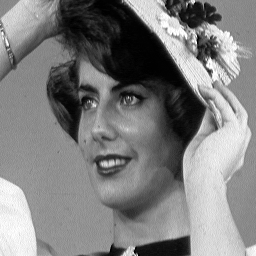
\includegraphics[width=1.1in]{imgs/Lena.png}
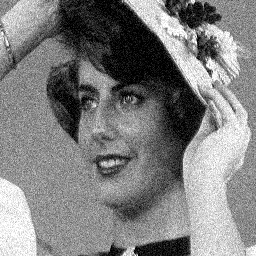
\includegraphics[width=1.1in]{imgs/Lenanoise.png}
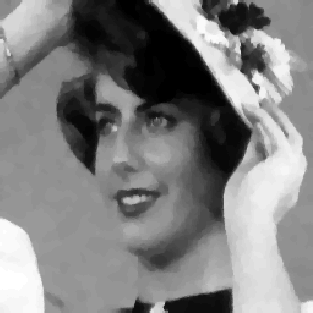
\includegraphics[width=1.1in]{imgs/Lenadenoise11.png}
\caption{Gaussian:$\sigma=0.02$ image}
\label{1:2}
\end{minipage}
\begin{minipage}[t]{0.5\textwidth}
\centering
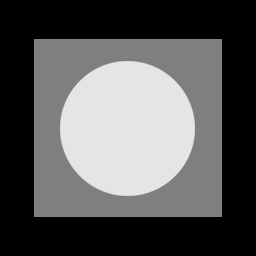
\includegraphics[width=1.1in]{imgs/gaussian-original.png}
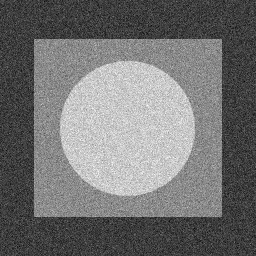
\includegraphics[width=1.1in]{imgs/gaussian-noise.png}

\includegraphics[width=1.1in]{imgs/gaussian-denoise11.png}
\end{minipage}
\end{figure} 
\end{frame}

\section{TV denoising - Chambolle's Projection Algorithm}

%
\begin{frame}
\frametitle{Chambolle's Projection Algorithm} 
\begin{itemize}
\item When $\phi(t)=t$ and $R$ is the identity operator, Chambolle has remarked that the minimization of the total variation can be viewed as a projection problem on a suitable convex set.
\item Chambolle and Lions proved that the following unconstrained minimization problem is referred to as the ROF model:
\newcommand{\ud}{\mathrm{d}}
\begin{displaymath}
\min_{u\in BV(\Omega)}\int_\Omega|\nabla u(x)|\ud x+\frac{\lambda}{2}\parallel u-f \parallel_2^2
\end{displaymath}

for an adequate Lagrange multiplier $\lambda>0$.
\end{itemize}
\end{frame}

%
\begin{frame}
\frametitle{Chambolle's Projection Algorithm} 
\begin{itemize}
\newcommand{\ud}{\mathrm{d}}
\item We will denote by $u_{i,j},i,j=1,\ldots,N$, a discrete image and by $X=\mathbb{R}^{N^2}$ the set of all discrete images of size $N^2$.
\item $J(u)=\int_{\Omega}|\nabla u(x)|\ud x$. Here the functional $J$ is a discretization of the standard total variation.
\begin{displaymath}
J(u)=\sum_{1\leq i,j\leq N}|(\nabla u)_{i,j}|
\end{displaymath}

\item The problem we want to solve is
\begin{displaymath}
\min_{u\in X} \{J(u)+\frac{1}{2\lambda}\parallel u-f \parallel^2\}
\end{displaymath}

The unique minimizer of it is given by $u=f−P_{\lambda G}(f)$, where $P_{\lambda G}(f)$ is the $L^2$-orthogonal projection of $f$ on the set $\lambda G$.
\end{itemize}
\end{frame}

%
\begin{frame}
\frametitle{Chambolle's Projection Algorithm} 
\begin{itemize}
\item Computing the nonlinear projection $P_{\lambda G}(f)$ amounts to solving the following problem:
\begin{displaymath}
\min\{|\lambda \textrm{div} p-f\,|^2_{X\times X};p\in X\times X,|P_{i,j}|\leq1\; \forall i,j=1,\ldots,N\}
\end{displaymath}

For each $i,j$
\begin{displaymath}
-(\nabla(\lambda\textrm{div}\, p−f\,))_{i,j}+\alpha_{i,j}p_{i,j}=0
\end{displaymath}

\begin{displaymath}
\alpha_{i,j}=|(\nabla(\lambda\textrm{div}\, p−f\,))_{i,j}|
\end{displaymath}

\end{itemize}
\end{frame}

%
\begin{frame}
\frametitle{Chambolle's Projection Algorithm} 
Let $\tau>0$ be given and let $p^0=0$ be an initial guess. We compute $p^{n+1}_{i,j}$ as
\begin{displaymath}
p_{i,j}^{n+1}=p_{i,j}^n+\tau((\nabla(\textrm{div} p^n−f/\lambda))_{i,j}−|(\nabla(\textrm{div} p^n−f/\lambda))_{i,j}|p_{i,j}^{n+1})
\end{displaymath}

The final algorithm is described
\begin{displaymath}
p_{i,j}^{n+1}=\frac{p_{i,j}^n+\tau((\nabla(\textrm{div} p^n−f/\lambda)))_{i,j}}{1+\tau|(\nabla(\textrm{div} p^n−f/\lambda)))_{i,j}|}
\end{displaymath}

\begin{description}
\item [THEOREM] Let us assume that $0<\tau\leq\frac{1}{8}$. Then $\lambda \textrm{div} p^n$ converges to $P_{\lambda G}(f)$ as $n\rightarrow\infty$ .
\end{description}

\end{frame}

%
\begin{frame}
\frametitle{Chambolle's Projection Algorithm} 
\begin{itemize}
\item The gradient $\nabla:X\rightarrow X\times X$
\begin{displaymath}
(\nabla u)_{i,j}^1=\left \{\begin{array}{ll}
u(i+1,j)-u(i,j) & \textrm{if $i<N$}\\
0 & \textrm{if $i=N$}
\end{array}\right.
\end{displaymath}
\begin{displaymath}
(\nabla u)_{i,j}^2=\left \{\begin{array}{ll}
u(i,j+1)-u(i,j) & \textrm{if $j<N$}\\
0 & \textrm{if $j=N$}
\end{array}\right.
\end{displaymath}

\end{itemize}
\end{frame}

\begin{frame}
\frametitle{Chambolle's Projection Algorithm} 
\begin{itemize}
\item The divergence operator defined by analogy with the continuous case by div=$−\nabla^*$, where $\nabla^*$ is the adjoint of $\nabla$. 
\begin{displaymath}
(\textrm{div}\,p)_{i,j}=(\textrm{div}\, p)_{i,j}^1+(\textrm{div}\, p)_{i,j}^2
\end{displaymath}
\begin{displaymath}
(\textrm{div}\, p)_{i,j}^1=\left \{\begin{array}{ll}
p(i,j)^1-p(i-1,j)^1 & \textrm{if $1<i<N$}\\
p(i,j)^1 & \textrm{if $i=1$}\\
-p(i-1,j)^1 & \textrm{if $i=N$}
\end{array}\right.
\end{displaymath}
\begin{displaymath}
(\textrm{div}\, p)_{i,j}^2=\left \{\begin{array}{ll}
p(i,j)^2-p(i,j-1)^2 & \textrm{if $1<j<N$}\\
p(i,j)^2 & \textrm{if $j=1$}\\
-p(i,j-1)^2 & \textrm{if $j=N$}
\end{array}\right.
\end{displaymath}

\end{itemize}
\end{frame}

%
\begin{frame}
\lstinputlisting{./code/proj.m}
\end{frame}

%
\begin{frame}
\lstinputlisting{./code/div.m}
\end{frame}

%
\begin{frame}
\lstinputlisting{./code/grad.m}
\end{frame}

%
\begin{frame}
\begin{figure}[!ht]
\begin{minipage}[t]{0.5\textwidth}
\centering
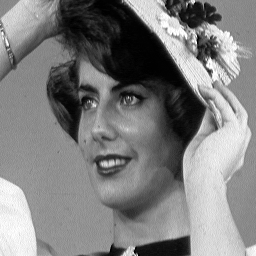
\includegraphics[width=1.1in]{imgs/Lena.png}
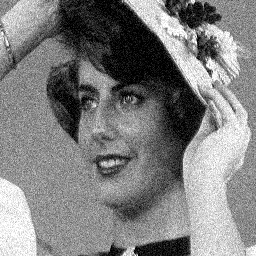
\includegraphics[width=1.1in]{imgs/Lenanoise.png}
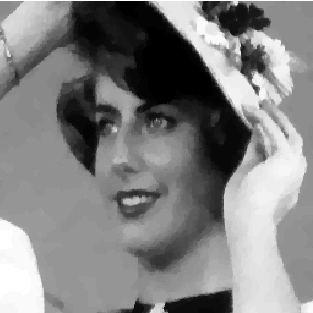
\includegraphics[width=1.1in]{imgs/Lenadenoise2.png}
\end{minipage}
\begin{minipage}[t]{0.5\textwidth}
\centering
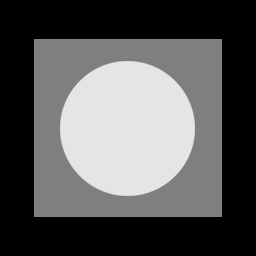
\includegraphics[width=1.1in]{imgs/gaussian-original.png}
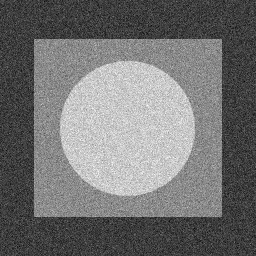
\includegraphics[width=1.1in]{imgs/gaussian-noise.png}

\includegraphics[width=1.1in]{imgs/gaussian-denoise2.png}
\end{minipage}
\end{figure} 
\end{frame}

\end{document}
